% Plain-language summary of DT-GSK -- standalone, seven pages.
% Audience: a reader with no optimization background. Success test: they can
% read it once and then explain the work accurately to someone else.
%
% NOT part of the submission package and NOT hashed by
% papers/governance/main_manuscript_freeze_manifest.json. Every number and
% every scope statement is read from the frozen analysis bundles under
% papers/analysis/ or from the manuscript's own text -- none from recollection.
% A three-seat audit (fact accuracy / honesty balance / lay readability)
% checked the first draft; where this summary could be read as claiming more
% than the paper does, the paper wins. Those corrections are preserved here.
%
% Build:  pdflatex -interaction=nonstopmode DT-GSK-plain-summary.tex  (x2)
\documentclass[11pt,a4paper]{article}

\usepackage[T1]{fontenc}
\usepackage[utf8]{inputenc}
\usepackage[english]{babel}
\usepackage{lmodern}
\usepackage[margin=0.88in]{geometry}
\usepackage{microtype}
\usepackage{parskip}
\usepackage{booktabs}
\usepackage{array}
\usepackage{enumitem}
\usepackage{titlesec}
\usepackage{xcolor}
\usepackage{tikz}
\usetikzlibrary{shapes.geometric, arrows.meta, positioning, calc, fit,
  backgrounds}
\usepackage[most]{tcolorbox}
\usepackage{hyperref}
\hypersetup{colorlinks=true, linkcolor=black, urlcolor=blue, citecolor=black,
  pdftitle={DT-GSK in Plain Language}, pdfauthor={Mostafa Elsayed Masoud}}

\setlength{\parindent}{0pt}
\setlength{\parskip}{4.4pt plus 1pt minus 1pt}
\titleformat{\section}{\large\bfseries}{\thesection.}{0.5em}{}
\titlespacing*{\section}{0pt}{8pt}{3pt}
\titleformat{\subsection}{\normalsize\bfseries}{}{0em}{}
\titlespacing*{\subsection}{0pt}{6pt}{1pt}
\newcommand{\hl}[1]{\textbf{#1}}

\definecolor{boxblue}{RGB}{232,240,250}
\definecolor{boxedge}{RGB}{70,110,160}
\definecolor{boxgrey}{RGB}{242,242,242}
\definecolor{boxgold}{RGB}{252,246,225}
\definecolor{goldedge}{RGB}{170,140,60}

\tikzset{
  dtbox/.style={rectangle, rounded corners=2pt, draw=boxedge, fill=boxblue,
    text width=7.4cm, align=center, minimum height=5.4mm, font=\footnotesize},
  dtgate/.style={rectangle, rounded corners=2pt, draw=goldedge, fill=boxgold,
    text width=6.6cm, align=center, minimum height=8mm, font=\small},
  dtterm/.style={rectangle, rounded corners=9pt, draw=black!65, fill=boxgrey,
    text width=3.2cm, align=center, minimum height=5mm, font=\footnotesize\bfseries},
  dtflow/.style={-{Latex[length=2mm]}, draw=black!65, thick},
}

\begin{document}

\begin{center}
{\LARGE\bfseries DT-GSK in Plain Language}\\[3pt]
{\large What it is, how it works, and what it proves}\\[7pt]
{\small Mostafa Elsayed Masoud \quad$\cdot$\quad Heba Sayed Mohamed Roshdy \quad$\cdot$\quad Ali Wagdy Mohamed}\\[2pt]
{\small Operations Research Department, Faculty of Graduate Studies for Statistical Research, Cairo University}\\[5pt]
{\footnotesize A seven-page companion to the paper \emph{DT-GSK: Dimension-Tiered Adaptive Control
and Deterministic Refinement for Gaining-Sharing Knowledge Optimization}.\\
Written for readers with no background in this field. Where this summary could
be read as claiming more than the paper does, the paper governs.}
\end{center}

\vspace{2pt}\hrule\vspace{6pt}

\section{The problem}

A lot of practical questions turn out to be the same question underneath:
\emph{out of a huge number of possibilities, which one is best?}

\begin{itemize}[leftmargin=1.2em, itemsep=1pt, topsep=3pt]
\item How should a power network be arranged so it wastes the least energy?
\item What shape makes a part as strong as possible for its weight?
\item Which combination of inputs makes a model match the real data most closely?
\end{itemize}

These problems are hard for two reasons. There is no formula that gives you the
answer. And there are far too many possibilities to try them all.

What you \emph{can} do is guess an answer, measure how good it is, and try
again. But each measurement is expensive: a simulation, a lab experiment, a
long calculation. So you only get a limited number of tries, and your job is to
spend them wisely.

This is called \hl{black-box optimization}. You can score an answer, but you
cannot look inside the problem and work out the solution directly.

\subsection{One word you need: ``unknowns''}

\hl{An ``unknown'' is one quantity you are allowed to change.} If you are
designing a beam and you can choose its length, width, and thickness, that
problem has three unknowns. Think of them as dials you can turn.

Some problems have 10 dials. Some have 1{,}000. \hl{That number is the key to
this whole paper.}

\subsection{How these methods work}

Most methods for this job work a bit like breeding plants.

\begin{enumerate}[leftmargin=1.4em, itemsep=1pt, topsep=3pt]
\item Start with a group of candidate answers.
\item Mix and adjust them to make new ones.
\item Test the new ones. Keep the better ones, drop the worse ones.
\item Repeat until you run out of tries.
\end{enumerate}

The skill is in step 2. Be too careful and you never discover anything new. Be
too wild and you never settle down and refine a good answer.

\section{The family this work builds on}

This project builds on a method called \hl{Gaining-Sharing Knowledge}, or GSK.
It copies the way people learn.

When you are new at something, you learn from people just ahead of you and just
behind you. Later, once you have some experience, you learn from the very best
people you can reach. GSK gives its candidate answers those same two modes: a
\hl{junior} mode that copies near neighbours, and a \hl{senior} mode that copies
the best and worst performers in the group.

Several improved versions of GSK have been published in recent years. Each one
adjusts how those two modes are tuned.

\subsection{The gap this paper found}

All of those versions share one habit. Each one settles on a single way of
behaving, and uses it for everything. \hl{The same dial settings are used whether
the problem has 10 unknowns or 1{,}000.}

That is a genuine weakness, because the size of a problem changes what a good
strategy looks like.

With 10 unknowns the search space is small enough to explore carefully, and
careful machinery pays off. With 1{,}000 unknowns that same machinery just burns
through the budget, while other tools, useless on a small problem, start to help
a lot.

\hl{One setting cannot be right for both.} That is the gap.

\section{What DT-GSK does differently}

DT-GSK changes its own machinery to match the size of the problem. That is what
``Dimension-Tiered'' means in its name.

\hl{Think of a gearbox with four gears:} under 20 unknowns, 20 to 49, 50 to 99,
and 100 or more.

One important detail. \hl{The gear is chosen once, before the search starts,
based purely on how many unknowns the problem has. It never changes during the
run.} A 60-unknown problem simply gets different parts switched on than a
15-unknown one does.

\begin{center}
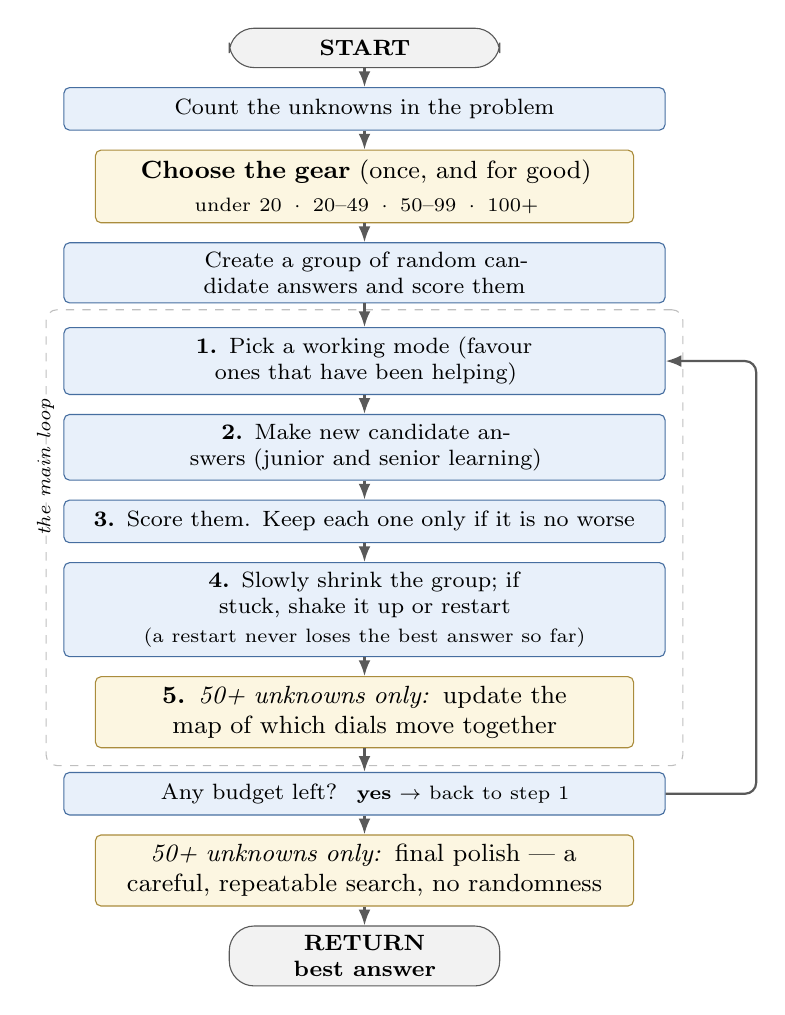
\begin{tikzpicture}[node distance=2.4mm]
\node[dtterm] (start) {START};
\node[dtbox, below=of start] (size) {Count the unknowns in the problem};
\node[dtgate, below=of size] (gear) {\textbf{Choose the gear} (once, and for good)\\[1pt]
  \scriptsize under 20 \,$\cdot$\, 20--49 \,$\cdot$\, 50--99 \,$\cdot$\, 100+};
\node[dtbox, below=of gear] (init) {Create a group of random candidate answers
  and score them};

\node[dtbox, below=3mm of init] (mode) {\textbf{1.} Pick a working mode
  (favour ones that have been helping)};
\node[dtbox, below=of mode] (make) {\textbf{2.} Make new candidate answers
  (junior and senior learning)};
\node[dtbox, below=of make] (test) {\textbf{3.} Score them. Keep each one only
  if it is no worse};
\node[dtbox, below=of test] (shrink) {\textbf{4.} Slowly shrink the group;
  if stuck, shake it up or restart\\[1pt]
  \scriptsize (a restart never loses the best answer so far)};
\node[dtgate, below=of shrink] (map) {\textbf{5.} \emph{50+ unknowns only:}
  update the map of which dials move together};

\node[dtbox, below=3mm of map] (budget) {Any budget left?
  \ \scriptsize\textbf{yes} $\rightarrow$ back to step 1};
\node[dtgate, below=of budget] (polish) {\emph{50+ unknowns only:} final polish
  --- a careful, repeatable search, no randomness};
\node[dtterm, below=of polish] (end) {RETURN best answer};

\draw[dtflow] (start)--(size);
\draw[dtflow] (size)--(gear);
\draw[dtflow] (gear)--(init);
\draw[dtflow] (init)--(mode);
\draw[dtflow] (mode)--(make);
\draw[dtflow] (make)--(test);
\draw[dtflow] (test)--(shrink);
\draw[dtflow] (shrink)--(map);
\draw[dtflow] (map)--(budget);
\draw[dtflow] (budget)--(polish);
\draw[dtflow] (polish)--(end);

\begin{scope}[on background layer]
\node[draw=black!25, dashed, rounded corners, fit=(mode)(map),
      inner sep=2.2mm, label={[font=\scriptsize\itshape, anchor=west,
      rotate=90, xshift=-1mm]west:the main loop}] {};
\end{scope}

\draw[dtflow, rounded corners]
  (budget.east) -- ++(1.15,0) |- (mode.east);
\end{tikzpicture}

{\footnotesize\textbf{Figure 1.} How DT-GSK runs. The two gold boxes are the
parts that only switch on for larger problems.}
\end{center}

\section{The three ideas inside it}

\subsection{Idea 1: machinery that tunes itself}

Instead of fixing its settings in advance, DT-GSK keeps several working modes
available and watches which ones are actually producing improvements. Modes that
help get picked more often. Modes that stop helping are set aside, but not
permanently, so a mode can come back if it becomes useful again.

It also shrinks its group of candidates over time: early on it spreads effort
wide, later it concentrates on refining what it has. And it has a safety net.
If progress stalls badly it restarts from fresh candidates while keeping the
best answer found so far, so \hl{a restart can never lose ground.}

\hl{This part runs at every problem size, including the smallest ones.}

\subsection{Idea 2: a careful, repeatable finish}

Most methods in this family finish the way they started: randomly. DT-GSK does
something different at the end. It stops guessing and runs a \hl{systematic
search} around its best answer. Step one way, test. Step the other way, test.
Shrink the step. Repeat. There is no randomness in it at all.

\hl{This only switches on from 50 unknowns upward}, and it runs once, in the last
few percent of the budget.

It helps in a practical way too. A random finish gives a slightly different
answer every time you run it. A repeatable finish gives exactly the same answer
every time --- \emph{as long as you run it on the same computer setup the study
used.} The paper is careful to say this is not promised across different
hardware.

\subsection{Idea 3: a memory of what worked (the honest one)}

The third idea is more experimental. While it searches, DT-GSK notices which
\emph{pairs} of dials tend to improve together, and builds a simple map of those
relationships. It uses the map to decide which dials to change as a group, and to
aim the final polish. \hl{Like the polish, it only switches on from 50 unknowns
up.}

Building the map needs no extra measurements of the problem. It is put together
from measurements the method was already taking.

But it is not free. Switching it on made runs roughly \hl{30 to 57 percent
slower} in the authors' own timings.

And here the paper says something you rarely see. \hl{When this memory was
tested on its own, it produced no measurable benefit.} The authors ran that test
specifically to find out, got a negative answer, and put it in the paper's
abstract and conclusions instead of leaving it out. So this component cost real
computing time and bought nothing they could detect --- and they published that.

\section{The method, step by step}

Here is the whole method in plain steps. ``D'' just means the number of unknowns.

\begin{tcolorbox}[colback=boxgrey, colframe=black!45, boxrule=0.4pt,
  arc=2pt, left=3.5mm, right=2.5mm, top=2mm, bottom=2mm]
{\small
\textbf{INPUT:} the problem, its number of unknowns $D$, and a fixed budget of
tests.\\[3pt]

\textbf{1. Choose the gear} from $D$, once, before starting:\\
\hspace*{4mm}$D < 20$ \ \ \ \ \ $\rightarrow$ self-tuning machinery only\\
\hspace*{4mm}$D = 20\!-\!49$ \ \ $\rightarrow$ the above, plus an extra working mode\\
\hspace*{4mm}$D = 50\!-\!99$ \ \ $\rightarrow$ the above, plus the pair-map and the final polish\\
\hspace*{4mm}$D \geq 100$ \ \ \ $\rightarrow$ the above, plus extra protections for big problems\\[3pt]

\textbf{2. Set up.} Create $5 \times D$ random candidate answers. Score them all.\\[3pt]

\textbf{3. REPEAT until the budget is nearly spent:}\\
\hspace*{4mm}\textbf{a.} Pick a working mode, favouring ones that have been helping lately.\\
\hspace*{4mm}\textbf{b.} For each candidate, build one new trial answer:\\
\hspace*{9mm}$\cdot$ \emph{junior} --- copy from near neighbours\\
\hspace*{9mm}$\cdot$ \emph{senior} --- copy from the best and the worst\\
\hspace*{4mm}\textbf{c.} Score each trial. Keep it only if it is no worse than what it replaces.\\
\hspace*{4mm}\textbf{d.} Slightly shrink the group of candidates.\\
\hspace*{4mm}\textbf{e.} \emph{If $D \geq 50$:} update the map of which dials move together.\\
\hspace*{4mm}\textbf{f.} If progress has stalled: shake up the worst candidates. If it is\\
\hspace*{9mm}still stuck, restart --- but never lose the best answer found.\\[3pt]

\textbf{4. Final polish} \emph{(only if $D \geq 50$).} Spend the last few percent
of the budget\\
\hspace*{4mm}searching carefully around the best answer: step along a direction,\\
\hspace*{4mm}test, shrink the step, repeat. No randomness.\\[3pt]

\textbf{5. RETURN} the best answer seen at any point.
}
\end{tcolorbox}

Notice that steps 1 and 4 are what make this method different from the rest of
its family. Everything else is a refinement of ideas the family already had.

\section{How it was tested}

A claim like ``this method is better'' is only as strong as the comparison
behind it. This study was built so the comparison can be checked.

\subsection{Who competed}

Seven methods: DT-GSK plus \hl{six published methods from the same family}
(GSK, AGSK, APGSK, FDB-AGSK, ATMALS-GSK, and eGSK).

The six were not compared using numbers copied out of their original papers.
They were re-built and re-run inside this project, so every method faced exactly
the same problems and the same budget.

\hl{One disclosure the paper makes, and this summary repeats:} five of the six
competing methods were written or co-written by two of this paper's own authors,
including the original GSK. No method from outside this family is included in any
comparison.

\subsection{On what}

Five standard test collections that this research community uses. That came to
12{,}265 runs per method, or about \hl{86{,}000 runs in total}.

\begin{center}
\small
\begin{tabular}{@{}llll@{}}
\toprule
\textbf{Collection} & \textbf{What is in it} & \textbf{Sizes} & \textbf{Runs each} \\
\midrule
CEC2017 & 29 mathematical test problems & 10--100 unknowns & 51 \\
CEC2011 & 22 real-world problem descriptions & as given & 25 \\
CEC2013 & 28 mathematical test problems & 10--50 unknowns & 51 \\
CEC2020 & 10 problems, all small & 5--20 unknowns & 30 \\
CEC2013LSGO & 15 very large problems & 1{,}000 (two at 905) & 25 \\
\bottomrule
\end{tabular}
\end{center}

\subsection{Under what rules}

\begin{itemize}[leftmargin=1.2em, itemsep=2pt, topsep=3pt]
\item \hl{Equal budget.} Every method got exactly the same number of tests on
      every problem. Nobody got extra tries.
\item \hl{Matched starting points.} On each problem, every method used the same
      recorded random seed. The six older methods also started from an identical
      set of candidate answers. \hl{DT-GSK is the one exception the paper
      documents}: it builds its own starting set from the same seed, because it
      uses a different group size. The authors flag this as the one place the
      comparison is not perfectly matched.
\item \hl{An analysis plan written in advance --- for one collection.} For
      CEC2020, the authors wrote down exactly how they would analyse the results
      \emph{before} running them, and saved that plan with a timestamp. That
      makes it impossible to pick a flattering analysis afterwards. But this
      covers CEC2020 only. The other four collections had no plan committed in
      advance, and on the very large problems the authors say they had already
      seen the standings before writing their plan.
\end{itemize}

\subsection{How the scores were compared}

Raw scores vary enormously from problem to problem, so the study uses
\hl{average rank} instead. On each problem the seven methods are ranked 1st to
7th. Those positions are then averaged.

\begin{center}
\small
\begin{tabular}{@{}cl@{}}
\toprule
\textbf{Average rank} & \textbf{Meaning} \\
\midrule
1.0 & won every single problem \\
2.5 & usually near the top \\
4.0 & exactly middle of the pack \\
7.0 & lost every single problem \\
\bottomrule
\end{tabular}
\end{center}

Separate statistical tests then ask whether a gap is real or could just be luck.
\hl{Important: the average ranks below are descriptive summaries. No statistical
test is attached to them.}

\section{What they found}

\begin{center}
\small
\begin{tabular}{@{}p{2.1cm}p{5.4cm}p{3.0cm}c@{}}
\toprule
\textbf{Collection} & \textbf{What kind of test it is} & \textbf{DT-GSK's place} & \textbf{Avg.\ rank} \\
\midrule
CEC2017 & the collection its settings were chosen on, so the least independent of the five & \hl{1st of 7} & 2.48 \\
CEC2013 & a second check, but not an independent benchmark & \hl{1st of 7} & 2.80 \\
CEC2013LSGO & added later, exploratory; standings were looked at before the plan was written & tied 1st with AGSK & 3.13 \\
CEC2011 & real-world problem descriptions & 2nd, behind eGSK & 3.36 \\
CEC2020 & the one test planned in advance & \hl{4th of 7} (AGSK 1st, 2.09) & 4.11 \\
\bottomrule
\end{tabular}
\end{center}

In short: first on two collections, tied first on one, second on one, and fourth
on one.

\subsection{Reading the good results fairly}

Three things limit them.

\hl{Who it was compared against.} DT-GSK was tested against its own family, not
against the strongest optimization methods in the world. The paper makes no
claim about the wider field. On the 1{,}000-unknown problems it says so plainly:
specialist large-scale methods report much better published results than any
method in this family, DT-GSK included.

\hl{No test is attached.} The first places are average-rank summaries. Against
its closest rival, eGSK, DT-GSK's lead on the main collection is small enough
that the statistical tests cannot call it real at any problem size.

\hl{Where the settings came from.} CEC2017 gave the headline first place, and
CEC2017 is also the collection the authors used to choose DT-GSK's settings.
Six candidate setups were compared on it before one was frozen. So that result
should be read as performance on home ground, not as a fresh test.

The tied first place on the very large problems is the weakest of the three. On
that collection the tests cannot tell six of the seven methods apart at all.

\subsection{Reading the bad results fairly}

\hl{Second place on the real-world set.} On CEC2011, eGSK beat DT-GSK, and the
statistical test says that gap is real. One clarification about what CEC2011 is:
these are engineering problems taken from practice and turned into a standard
benchmark. That shows the method has been tried on a broad range of problem
types. It is not evidence of how it would perform in an actual deployment, and
the paper is careful about that distinction.

\hl{Fourth place on the small problems.} On CEC2020, where every problem has 20
or fewer unknowns, DT-GSK finished fourth of seven. The reason is built into the
design: its two size-gated parts, the pair-map and the final polish, do not
switch on until 50 unknowns. So here it competes without the machinery that wins
it results higher up. Its self-tuning machinery is still running, so this is a
real result about the method as it is configured, not a fluke.

The authors had written down, before running it, that they expected DT-GSK
\emph{not} to lead this collection. That same plan also required them to report
the outcome as a real finding rather than explain it away.

\hl{Three confirmed losses, not one.} CEC2011 is the only confirmed loss for a
whole collection. But it is not the only one. On CEC2020 at 20 unknowns, the same
test confirms that both AGSK and FDB-AGSK beat DT-GSK. Those two sit in the
study's strongest category of evidence, because CEC2020 is the collection that
was planned in advance.

\subsection{The shape of the strength}

The advantage is \hl{tiered, and it is not simply ``the bigger the better''.}

Across the two mathematical collections covering 10 to 100 unknowns, DT-GSK
leads at every size except 30, where it drops to second on CEC2017 and third on
CEC2013. On the small collection it leads at none of the four sizes. On the
real-world set it is second. \hl{Its strength is concentrated at 50 unknowns and
above.}

\section{Limits, and why you can check all this}

\subsection{What the paper does not claim}

\begin{itemize}[leftmargin=1.2em, itemsep=2pt, topsep=3pt]
\item It does not claim DT-GSK is the best optimization method available. It does
      not even claim DT-GSK is the best method in its own family overall. The
      paper reports its standing size by size rather than as a single verdict,
      and other family members beat it at some sizes and on the real-world set.
\item It does not claim the pair-map works. The direct test of it came back
      negative, and that is reported.
\item It does not claim to run faster. One competitor, eGSK, could only be
      rebuilt using a substitute for one internal solver. That part uses some of
      the same budget and can change the answer it returns, so the eGSK results
      here belong to this rebuild rather than to the published original. That
      cuts both ways: eGSK is the method that beats DT-GSK on the real-world set.
\item It does not claim the settings are the best possible. They were frozen and
      never re-tuned per problem, with one disclosed exception: two values were
      added for the very-large-problem collection after results on it already
      existed, so that result is not claimed to be blind to its own outcome.
\end{itemize}

\subsection{Why the numbers can be checked}

The unusual thing about this project is not the method. It is the paper trail.

\begin{itemize}[leftmargin=1.2em, itemsep=2pt, topsep=3pt]
\item \hl{Every run is kept}, stored in read-only frozen data sets rather than
      summarised away.
\item \hl{Results can be reproduced in the setup the authors describe.} The
      random number streams are pinned to recorded starting seeds, so re-running
      DT-GSK on a matching setup gives back the same numbers, not merely similar
      ones. This promise is made for DT-GSK and this project's own analysis
      tools.
\item \hl{Every number in the paper can be traced} back to the data file it came
      from, and automatic checks confirm the paper and the data still agree.
\item \hl{The negative results are published too}: the component that did not
      work, the computing time it cost, the loss on the real-world set, the
      fourth place, and the two confirmed losses at 20 unknowns.
\end{itemize}

\subsection{If you have thirty seconds to explain it}

\begin{tcolorbox}[colback=boxblue, colframe=boxedge, boxrule=0.5pt, arc=2pt,
  left=3mm, right=3mm, top=2.5mm, bottom=2.5mm]
It is a search method for hard problems where you can test an answer but cannot
work out the best one directly. Its main idea is that it picks its own machinery
based on how big the problem is, like choosing a gear before you set off, instead
of using one setting for everything. Above a certain size it also finishes with a
careful, repeatable polish rather than a random one. It was tested against six
other published methods from \emph{its own family} --- not against the strongest
methods in the field, a comparison the paper does not make --- across five
standard test collections with equal budgets. It came first on two, tied first on
one, second on one, and fourth on one. It is weakest on small problems, where its
size-gated machinery is switched off by design, and it loses on the real-world
set. One of its three components was tested on its own, cost 30 to 57 percent
more computing time, and showed no measurable benefit --- and the authors
published that result instead of leaving it out.
\end{tcolorbox}

\vspace{3pt}\hrule\vspace{3pt}
{\footnotesize
\emph{Sources.} All standings are the descriptive average ranks in the project's
frozen analysis files. Protocol figures and every scope statement come from the
paper itself. This is a companion document and is not part of the submitted
package. For the full method, the statistical tests, and the complete results,
see the paper and its Supplementary Material.}

\end{document}
